\section{Auswertung}
\label{sec:Auswertung}

\subsection{Ausmessung des Acryl Blocks mittels A-Scan}

Die Ausmessung mittels einer Schieblehre führt zu den Daten, die in Tabelle \ref{tab:mess1} 
dargestellt sind. 

\begin{table}
  \centering
  \caption{Messdaten des Acrylblocks}
  \label{tab:mess1}
  \sisetup{table-format=2.1}
  \begin{tabular}{c c}
  \toprule
  &$s \,/\, \si{\centi\metre}$\\
  \midrule 
  Länge  & 15,000\\
  Höhe   &  8,035\\
  Breite &  3,995\\
  \bottomrule
  \end{tabular}
  \end{table}

Der A-Scan liefert Laufzeiten, die den Ort der Fehlstellen angeben. Bei diesen ist zu beachten, 
dass zunächst die Laufzeit des Koppelmaterial und der Schutzschicht von den Ergebnissen 
subtrahiert werden müssen. Die Schutzschicht hat eine Dicke von $\SI{0.2}{\centi\meter}$. \\
Aus diesen Laufzeiten werden die Abstände $D_\text{oben}$ der oberen Enden der Fehlstellen zu dem oberen Ende des 
Blocks, sowie die Abstände $D_\text{unten}$ der unteren Enden der Fehlstellen zu dem unteren Ende des Blocks 
bestimmt. Für diese Berechnung wird eine Phasengeschwindigkeit in Acryl von $\SI{2730}{\meter\per\second}$ im 
Weg-Zeit-Gesetz verwendet [2]. Zusammen mit der ermittelten Höhe des Blockes ergeben sich die Durchmesser 
der Fehlstellen $D_\text{Loch}$. Diese Werte finden sich in Tabelle \ref{tab:mess2}.

\begin{table}
\centering
\caption{Messdaten der Tiefenmessungen des Acrylblocks}
\label{tab:mess2}
\sisetup{table-format=2.1}
\begin{tabular}{c c c c c c}
\toprule
Stelle & $t_1 \,/\, \si{\micro\second}$ & $t_2 \,/\, \si{\micro\second}$ &$D_\text{oben} \,/\, \si{\centi\meter}$&$D_\text{unten} \,/\, \si{\centi\meter}$ & $D_\text{Loch} \,/\, \si{\milli\meter}$\\
\midrule 
9 & 48,5 & 14,1 & 6,25 & 1,56 & 2,25 \\
8 & 42,6 & 19,6 & 5,44 & 2,31 & 2,80\\
7 & 36,6 & 25,1 & 4,63 & 3,06 & 3,48\\
6 & 30,2 & 30,5 & 3,75 & 3,80 & 4,85\\
5 & 24,3 & 36,3 & 2,95 & 4,59 & 4,98\\
4 & 18,6 & 42,0 & 2,17 & 5,37 & 4,98\\
3 & 12,7 & 47,9 & 1,37 & 6,17 & 4,98\\
\bottomrule
\end{tabular}
\end{table}

Eine Aufnahme eines solchen A-Scans ist in Abbildung  zu sehen. 

\begin{figure}
  \centering
  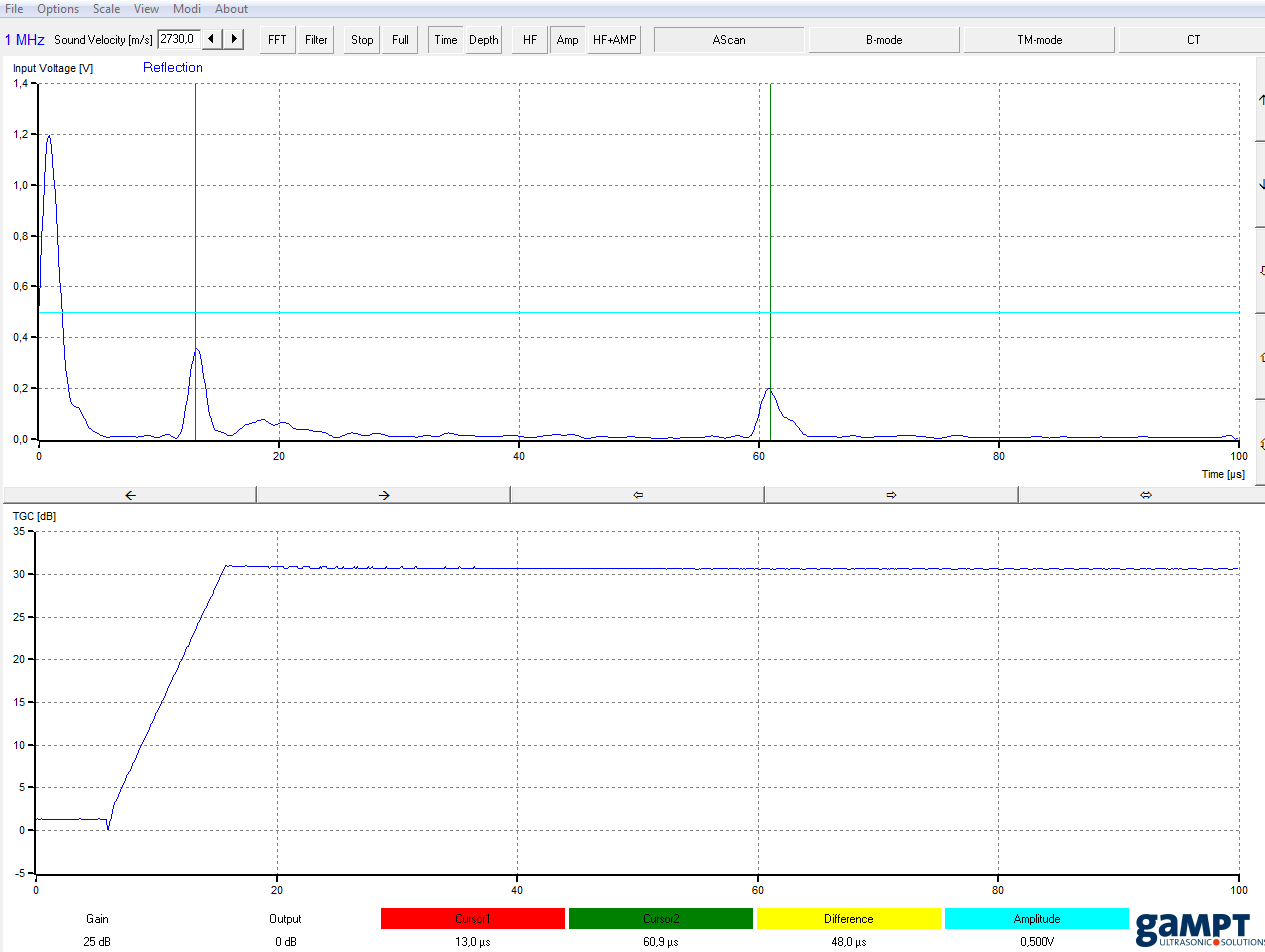
\includegraphics[scale=0.3]{content/Ascan.PNG}
  \caption{Beispielaufnahme eines A-Scans.}
  \label{fig:Ascan}
\end{figure}

Außerdem sollten die Fehlstellen 1 und 2 genauer untersucht werden. Hierzu wurden sie mit verschiedenen 
Sonden unterschiedlicher Frequenz abgetastet. Die Ergebnisse sind in Abbildung \ref{fig:Ascanblau},
\ref{fig:Ascanrot} und \ref{Ascangruen} zu sehen.

\begin{figure}
  \centering
  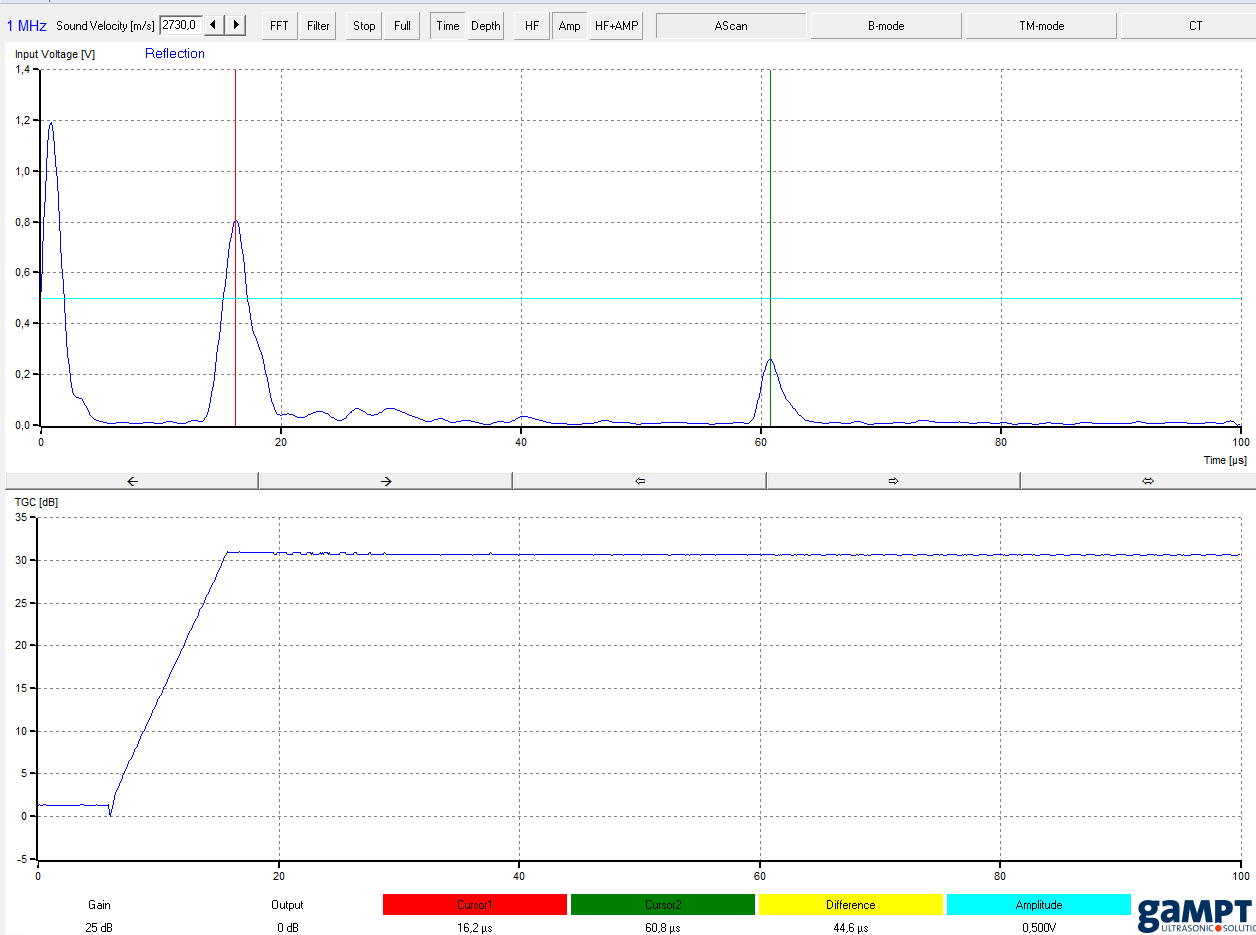
\includegraphics[scale=0.3]{content/blau-a-scan.PNG}
  \caption{Aufnahme eines A-Scans mit einer Ultraschallsonde mit $\SI{1}{\mega\hertz}$.}
  \label{fig:Ascanblau}
\end{figure}

\begin{figure}
  \centering
  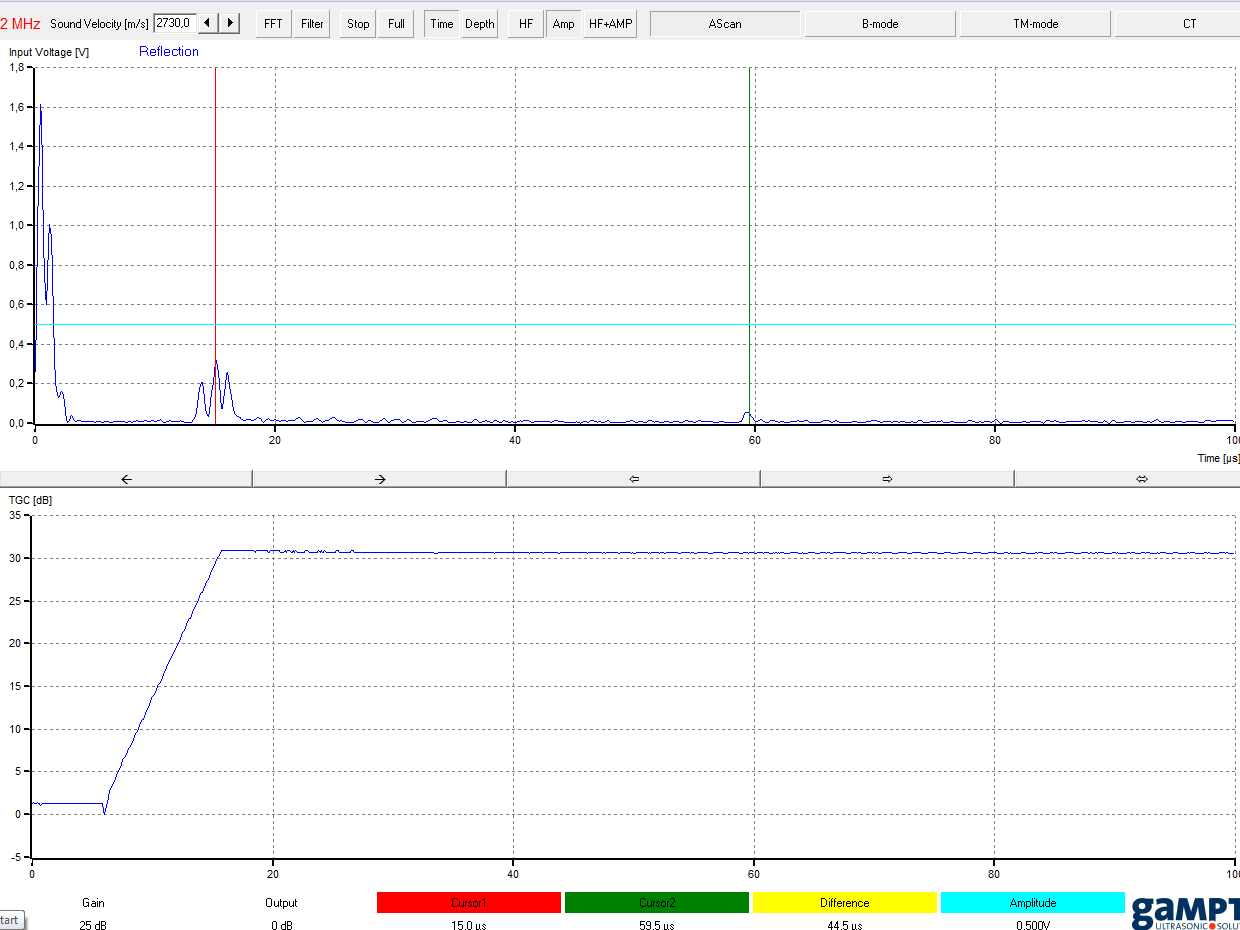
\includegraphics[scale=0.3]{content/rot-a-scan.PNG}
  \caption{Aufnahme eines A-Scans mit einer Ultraschallsonde mit $\SI{2}{\mega\hertz}$.}
  \label{fig:Ascanrot}
\end{figure}

\begin{figure}
  \centering
  \includegraphics[scale=0.3]{content/grün-a-scan.PNG}
  \caption{Aufnahme eines A-Scans mit einer Ultraschallsonde mit $\SI{4}{\mega\hertz}$.}
  \label{fig:Ascangruen}
\end{figure}

\subsection{Ausmessung des Acryl-Blocks mittels B-Scan}

Das Ergebnis des B-Scans von der Oberseite des Blocks ist in Abbildung \ref{fig:boben} wiedergegeben; das
des unteren in Abbildung \ref{fig:bunten}. 

\begin{figure}
  \centering
  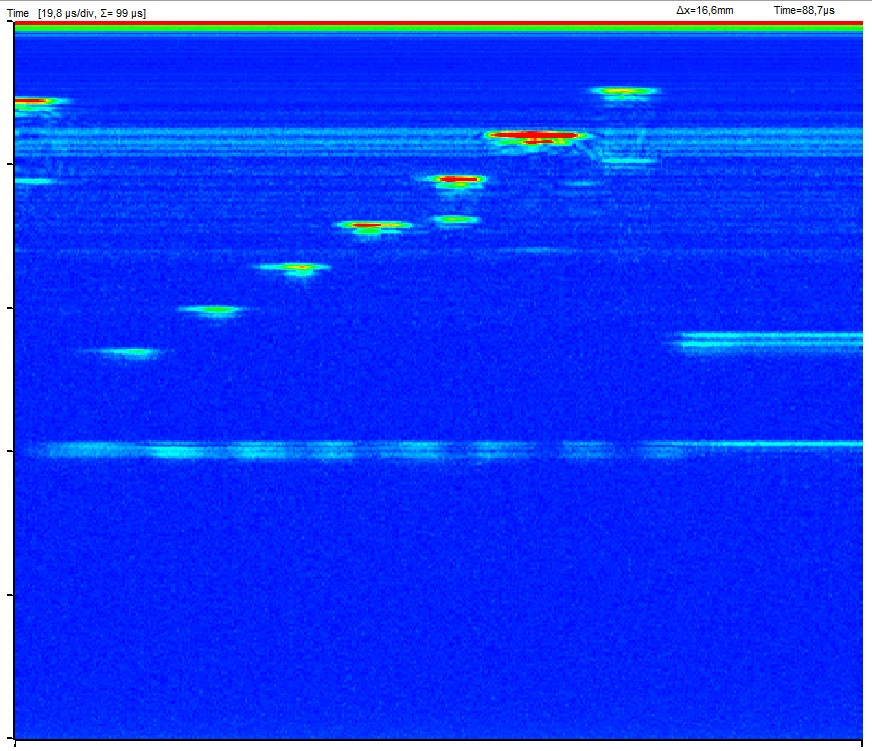
\includegraphics[scale=0.3]{content/bscan1.jpg}
  \caption{Ergebnis des B-Scans von oben.}
  \label{fig:boben}
\end{figure}

\begin{figure}
  \centering
  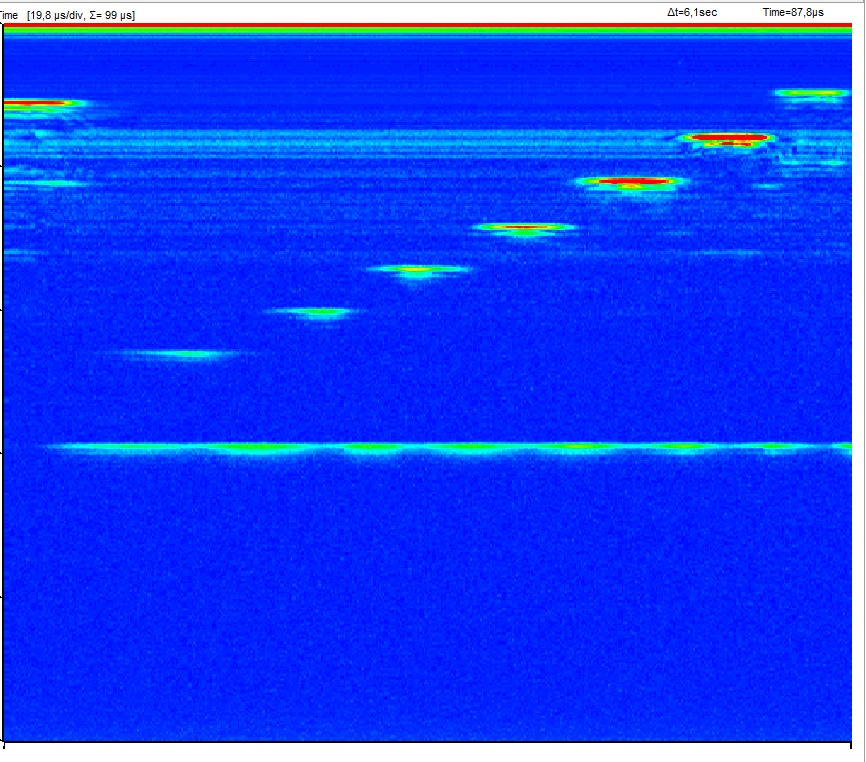
\includegraphics[scale=0.3]{content/bscan2.jpg}
  \caption{Ergebnis des B-Scans von unten.}
  \label{fig:bunten}
\end{figure}


Zunächst betrachten wir den Scan von oben. Aus diesem ergeben sich die Messwerte in Tabelle \ref{tab:mess3}.
Dabei werden wieder die Laufzeiten angegeben, deren Differenz und die daraus resultierenden 
Fehlstellendurchmesser.  

\begin{table}
\centering
\caption{Messdaten des ersten B-Scans.}
\label{tab:mess3}
\sisetup{table-format=2.1}
\begin{tabular}{c c c c c}
\toprule
Stelle & $t_\text{o} \,/\, \si{\micro\second}$ & $t_\text{u} \,/\, \si{\micro\second}$ &$\Delta t \,/\, \si{\micro\second}$ & $D_\text{Loch} \,/\, \si{\milli\meter}$\\
\midrule 
3 & 47,2 & 49,2 & 2,0 & 5,46\\
4 & 41,3 & 42,7 & 1,4 & 3,82\\
5 & 35,4 & 37,0 & 1,6 & 4,37\\
6 & 29,7 & 31,4 & 1,7 & 4,64\\
7 & 23,1 & 25,0 & 1,9 & 5,19\\
8 & 17,2 & 19,0 & 1,8 & 4,91\\
9 & 11,1 & 12,9 & 1,8 & 4,91\\
\bottomrule
\end{tabular}
\end{table}

Analog ergeben sich die Messwerte in Tabelle \ref{tab:mess4} für die zweite Messung mittels B-Scans.

\begin{table}
\centering
\caption{Messdaten des zweiten B-Scans.}
\label{tab:mess4}
\sisetup{table-format=2.1}
\begin{tabular}{c c c c c}
\toprule
Stelle & $t_\text{o} \,/\, \si{\micro\second}$ & $t_\text{u} \,/\, \si{\micro\second}$ &$\Delta t \,/\, \si{\micro\second}$ & $D_\text{Loch} \,/\, \si{\milli\meter}$\\
\midrule 
3 & 11,1 & 13,0 & 1,9 & 5,19\\
4 & 17,2 & 19,4 & 2,2 & 6,01\\
5 & 23,8 & 25,6 & 1,8 & 4,91\\
6 & 29,4 & 31,5 & 2,1 & 5,73\\
7 & 35,4 & 37,2 & 1,8 & 4,91\\
8 & 41,2 & 42,8 & 1,6 & 4,36\\
9 & 47,2 & 48,2 & 1,0 & 2,73\\
\bottomrule
\end{tabular}
\end{table}

Aus der Durchmessern werden die Mittelwerte bestimmt, welche in Tabelle \ref{tab:mess5} zu finden sind. 

\begin{table}
\centering
\caption{Gemittelte Durchmesser der Fehlstellen.}
\label{tab:mess5}
\sisetup{table-format=2.1}
\begin{tabular}{c c}
\toprule
Stelle & $D_\text{Loch} \,/\, \si{\milli\meter}$\\
\midrule 
3 & 5,325\\
4 & 4,915\\
5 & 4,640\\
6 & 5,185\\
7 & 5,050\\
8 & 4,635\\
9 & 3,820\\
\bottomrule
\end{tabular}
\end{table}

In der Diskussion werden die Ergebnisse aus A- und B-Scan verglichen.

\subsection{Bestimmung der Herzfrequenz und des Herzvolumens}

Ausgangspunkt der Messung der Herzfrequenz und des Herzvolumens ist der TM-Scan aus 
Abbildung \ref{fig:tm}. 

\begin{figure}
  \centering
  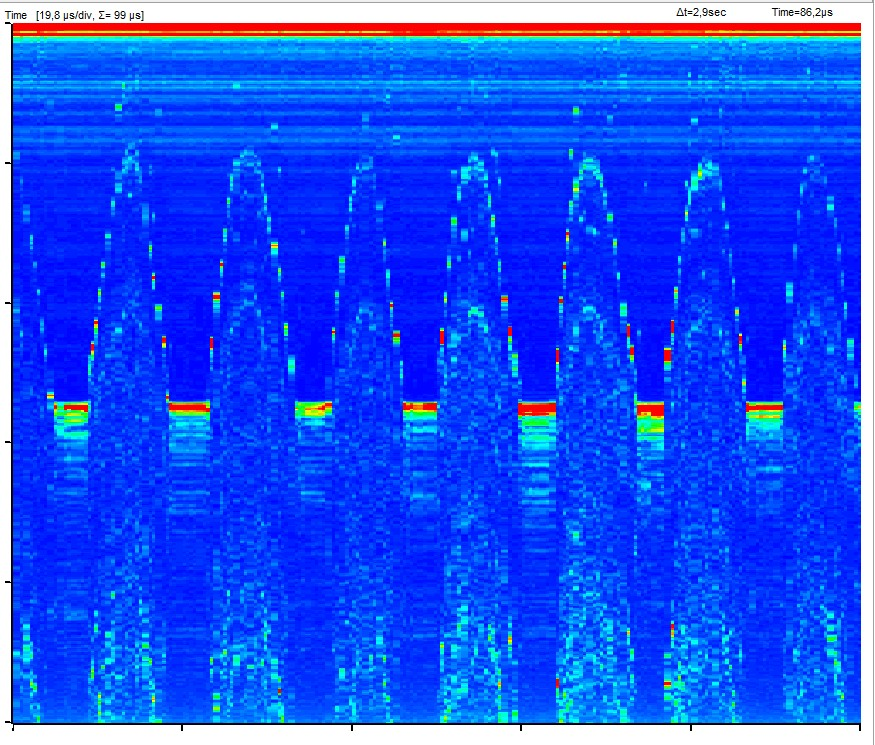
\includegraphics[scale=0.3]{content/tm.jpg}
  \caption{TM-Scan des schlagenden Herzmodells.}
  \label{fig:tm}
\end{figure}


Dabei ergibt sich die Amplitude zu

\begin{equation*}
A = \SI{54.8}{\micro\second}.
\end{equation*}

Der zeitliche Abstand der Herzschläge beträgt 

\begin{equation*}
\Delta t = \SI{1.4}{\second}.
\end{equation*}

Daraus ergibt sich eine Herzfrequenz von 

\begin{equation*}
f_\text{Herz} = \SI{0.71}{\hertz}.
\end{equation*}

Der endsystolischer Durchmesser (ESD) wird mit der Formel 

\begin{equation}
ESD = \frac{1}{2}\cdot c_\text{Wasser} \cdot A
\end{equation}

zu

\begin{equation*}
ESD = \SI{4.07}{\centi\meter}
\end{equation*}

bestimmt. Damit lässt sich nun das Herzvolumen, welches auf eine Kugel mittels 

\begin{equation*}
V_\text{Herz} = \frac{4\pi}{3}\left(\frac{ESD}{2}\right)³
\end{equation*}

genähert wird, zu 

\begin{equation*}
V_\text{Herz} = \SI{35.3}{\milli\liter}
\end{equation*}

berechnen. 